\documentclass[12pt]{article}
\usepackage{graphicx}
\usepackage{listings}
\begin{document}

\begin{titlepage}	
	\begin{center}	
		\Large{\textbf{Laboration 2}} \\
		[0.3 in]
		\large{\textit{DVA245}} \\
		[4.1 in]
	\end{center}

	\vspace{2in}
		
	\begin{flushright}
		\textsc{\large Aditya Subramanian} \\
		\textsc{\large Emil Willersjö Nyfelt} \\
		\today \\
	\end{flushright}
\end{titlepage}

\newpage
\section{Introduction}
\newpage
\section{max\_subsequence1}
\subsection{Algorithm analysis}
\begin{lstlisting}[language=Python]
def max_subsequence1(s):
    maxSum = 0                          # O(1)
    for i in range(len(s)):             # O(n)
        for j in range(i, len(s)):      # O(n^2)
            testSum = 0                 # O(1)
            for k in range(i, j+1):     # O(n^3)
                testSum += s[k]         # O(1)
            if testSum > maxSum:        # O(1)
                maxSum = testSum        # O(1)
    return maxSum                       # O(1)
\end{lstlisting}
The first for-loop traverses over the sequence once, thus yielding $O(n)$. The second for-loop  traverses over the sequence for each index $i$ making it $O(n^2)$. The last for-loop traverses the index $k$ over the interval given by $i$ and $j$. This will be done for every movement of $i$ and $j$ and thus making it $O(n^3)$ which is the order of this perticular algorithm. 
\subsection{Experimental results}
For the random sequence with lengths,
$n = [80,\,160,\, 320,\, 640,\, 1280]$ we have,
\begin{figure}[h]
\centering
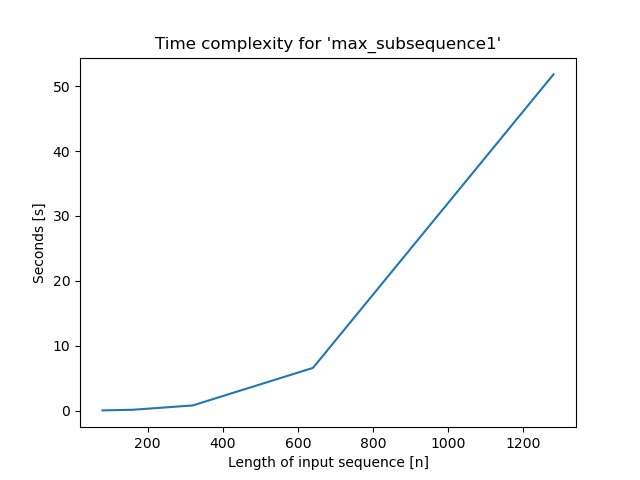
\includegraphics[scale=0.52]{ms1.png}
\end{figure}
\subsection{Discussion}
The experimental result concurs well with the analysis. For the length vector $n = [80,\,160,\, 320,\, 640,\, 1280]$ we get the corresponding time vector $ t = [0.0157,\,0.1106,\, 0.7791,\, 6.5699,\, 51.8298]$. Comparing the vectors, we can see that when the input doubles, the time roughly multiplies with eight which is consistent with a cubic function.  We see that the function $f(n) = an^3$ where $a$ is a constant, describes the running time with the input size as parameter.

\newpage
\section{max\_subsequence2}
\subsection{Algorithm analysis}
\begin{lstlisting}[language=Python]
def max_subsequence2(s):
    maxSum = 0                      # O(1)
    for i in range(len(s)):         # O(n)
        testSum = 0                 # O(1)
        for j in range(i, len(s)):  # O(n^2)
            testSum += s[j]         # O(1)
            if testSum > maxSum:    # O(1)
                maxSum = testSum    # O(1)
    return maxSum                   # O(1)
\end{lstlisting}
The first for-loop traverses over the sequence once, thus yielding $O(n)$. The second for-loop  traverses over the sequence for each index $i$ making it $O(n^2)$. The code inside the second for-loop is executed $n^2$ times and since no more complexity exists, the order of the algorithm is $O(n^2)$.
\subsection{Experimental results}
For the random sequence with lengths,
$n = [500,\,1000,\, 2000,\, 4000,\, 8000]$ we have,
\begin{figure}[h]
\centering
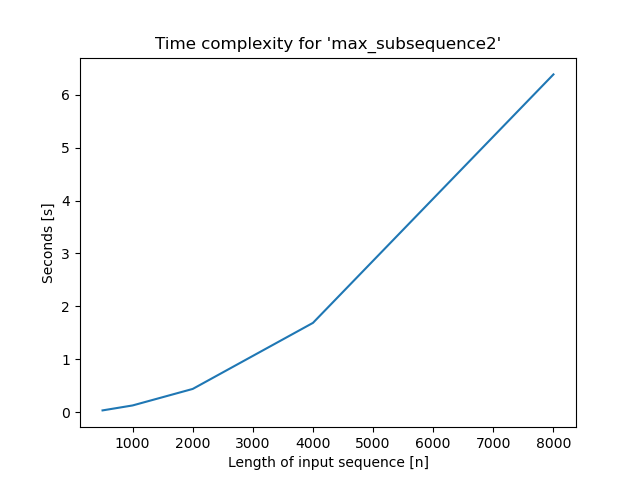
\includegraphics[scale=0.52]{ms2.png}
\end{figure}
\subsection{Discussion}
Again, the experimental result concurs well with the analysis. For the length vector $n = [500,\,1000,\, 2000,\, 4000,\, 8000]$ we get the corresponding time vector $ t = [0.0312,\,0.1250,\, 0.4374,\, 1.6867,\, 6.3862]$. Comparing the vectors, we can see that when the input doubles, the time roughly multiplies with four which is consistent with a square function.  We see that the function $f(n) = bn^2$ where $b$ is a constant, describes the running time with the input size as parameter.

\newpage
\section{max\_subsequence3}
\subsection{Algorithm analysis}
\begin{lstlisting}[language=Python]
def max_subsequence3(s):
    maxSum = 0                  # O(1)
    testSum = 0                 # O(1)
    for i in range(len(s)):     # O(n)
        testSum += s[i]         # O(1)
        if testSum > maxSum:    # O(1)
            maxSum = testSum    # O(1)
        if testSum < 0:         # O(1)
            testSum = 0         # O(1)
    return maxSum               # O(1)
\end{lstlisting}
The first for-loop traverses over the sequence once, thus yielding $O(n)$. The code in this for-loop is run $n$ times which makes this algorithm $O(n)$.

\subsection{Experimental results}
For the random sequence with lengths,
$n = [62500,\,125000,\, 250000,\, 500000,\, 1000000]$ we have,
\begin{figure}[h]
\centering
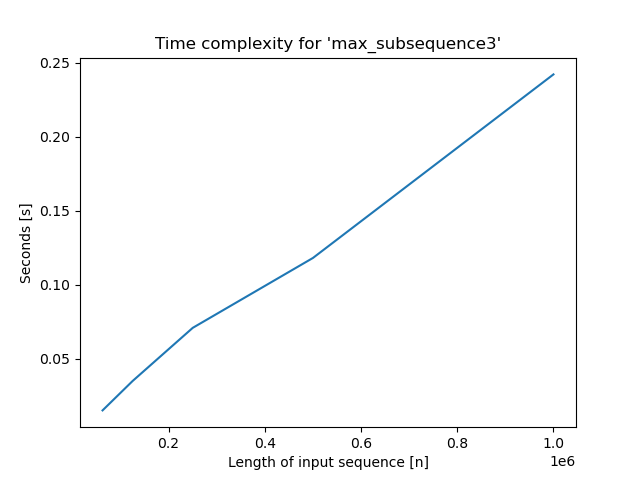
\includegraphics[scale=0.52]{ms3.png}
\end{figure}
\newpage
\subsection{Discussion}
This is also an expected result from the analysis. The graph is near linear showing that as the input size doubles, the running time doubles as well. For the length vector $n =  [62500,\,125000,\, 250000,\, 500000,\, 1000000]$ we get the corresponding time vector $ t = [0.0150,\,0.0346,\, 0.0708,\, 0.1181,\, 0.2421]$. comparing the vectors, we can see that the time indeed roughly doubles when the input doubles. The function $f(n) = cn$ where $c$ is a constant is thus a describing function.  
\section{Conclusion}
It is easy to solve for the constants $a,b,c$ but the important thing to see is that it will be different depending on the computer which runs the algorithm. A fast computer will yield a low constant since the algorithm will perform more calculations in less time.

\end{document}














